\documentclass{article}

\usepackage{graphicx}
\usepackage{tikz}
\usepackage{tikzsymbols}
\usetikzlibrary{calc,patterns,shapes.geometric}
\pagestyle{empty}
\usepackage[margin=0pt]{geometry}
\geometry{papersize={14in,12in}}

\def\centerarc[#1](#2)(#3:#4:#5){\draw[#1] ($(#2)+({#5*cos(#3)},{#5*sin(#3)})$) arc (#3:#4:#5);}

\begin{document}
	\begin{figure}
		\centering
		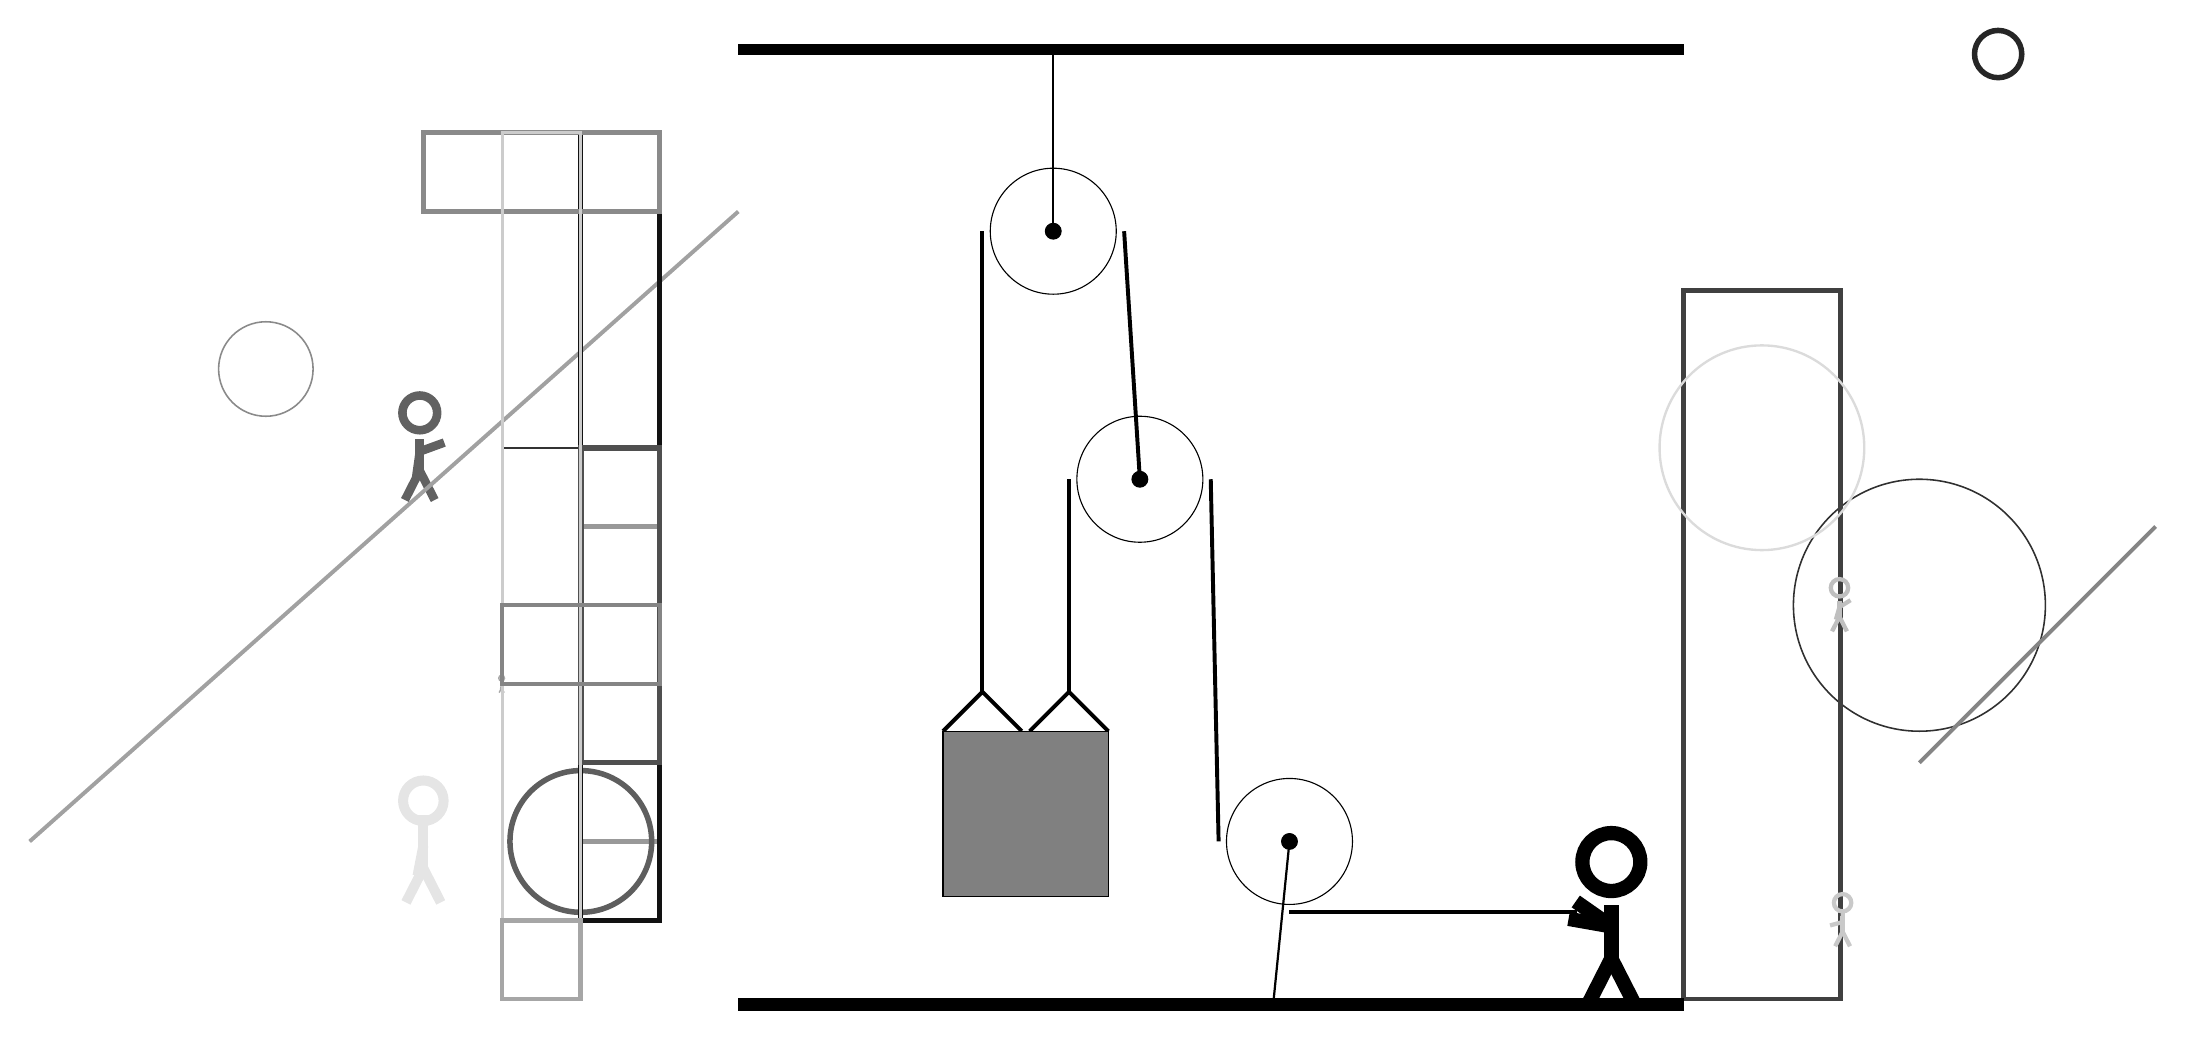
\begin{tikzpicture}
			%%%%% START %%%%%
			
			\draw[fill=black] (-2, 9) rectangle (10, 9.125);
			
			\draw (2, 6.75) circle (0.8);
			\draw[fill=black] (2, 6.75) circle (0.1);
			\draw[thick] (2, 6.75) -- (2, 9);
			
			\draw (3.1, 3.6) circle (0.8);
			\draw[fill=black] (3.1, 3.6) circle (0.1);
			
			\draw (5, -1) circle (0.8);
			\draw[fill=black] (5, -1) circle (0.1);
			\draw[thick] (5, -1) -- (4.8, -3);
			
			\draw[line width = 0.5mm]  (0.6, 0.4) -- (1.1, 0.9) -- (1.6, 0.4);
			\draw[line width = 0.5mm]  (1.7, 0.4) -- (2.2, 0.9) -- (2.7, 0.4);
			\draw[fill=black!50] (0.6, 0.4) rectangle (2.7, -1.7);
			
			\node[line width=0.7mm, color=black!10] at (-6, -1) {\Strichmaxerl[7][79][90]};
			
			\draw [line width=0.2mm, color=black!81](13, 2) circle (1.6);
			\draw[line width=0.6mm, color=black!75] (12, 6) rectangle (10, -3);
			\draw[line width=0.6mm, color=black!40] (-3, -1) rectangle (-4, 3);
			\node[line width=0.2mm, color=black!25] at (12, 2) {\Strichmaxerl[3][74][32]};
			
			\node[line width=0.5mm, color=black!62] at (-6, 4) {\Strichmaxerl[6][82][20]};
			\draw [line width=0.3mm, color=black!14](11, 4) circle (1.3);
			
			\draw [line width=0.7mm, color=black!63](-4, -1) circle (0.9);
			\draw[line width=0.5mm, color=black!37](-2, 7) -- (-11, -1);
			\node[line width=0.2mm, color=black!21] at (12, -2) {\Strichmaxerl[3][15][89]};
			\draw[line width=0.6mm, color=black!93] (-4, 8) rectangle (-3, -2);
			
			\draw[line width=0.5mm, color=black!48](13, 0) -- (16, 3);
			\draw[line width=0.6mm, color=black!46] (-3, 7) rectangle (-6, 8);
			
			\draw[line width=0.3mm, color=black!80] (-4, 4) rectangle (-5, 1);
			\draw [line width=0.2mm, color=black!46](-8, 5) circle (0.6);
			\node[line width=0.3mm, color=black!34] at (-5, 1) {\Strichmaxerl[1][76][29]};
			
			\draw[line width=0.7mm, color=black!69] (-4, 0) rectangle (-3, 4);
			\draw[line width=0.4mm, color=black!20] (-4, 8) rectangle (-5, -3);
			\draw[line width=0.6mm, color=black!35] (-4, -2) rectangle (-5, -3);
			\draw[line width=0.5mm, color=black!48] (-3, 1) rectangle (-5, 2);
			\draw [line width=0.7mm, color=black!85](14, 9) circle (0.3);
			
			
			\draw[line width = 0.5mm] (1.1, 6.75) -- (1.1, 0.9);
			\centerarc[line width = 0.5mm](2, 6.75)(0:180:0.9);
			\draw[line width = 0.5mm] (2.9, 6.75) -- (3.1, 3.6);
			\draw[line width = 0.5mm] (2.2, 3.6) -- (2.2, 0.9);
			\centerarc[line width = 0.5mm](3.1, 3.6)(0:180:0.9);
			\draw[line width = 0.5mm] (4.0, 3.6) -- (4.1, -1);
			\centerarc[line width = 0.5mm](5, -1)(180:270:0.9);
			\draw[line width = 0.5mm] (5, -1.9) -- (8.65, -1.9);
			
			\node at (9, -2) {\Strichmaxerl[10][-35][170]};
			
			\draw[fill=black] (-2, -3) rectangle (10, -3.15);
			
			%%%%% END %%%%%
		\end{tikzpicture}
	\end{figure}	
\end{document}